\let\negmedspace\undefined
\let\negthickspace\undefined
\documentclass[journal]{IEEEtran}
\usepackage[a5paper, margin=10mm, onecolumn]{geometry}
%\usepackage{lmodern} % Ensure lmodern is loaded for pdflatex
\usepackage{tfrupee} % Include tfrupee package

\setlength{\headheight}{1cm} % Set the height of the header box
\setlength{\headsep}{0mm}     % Set the distance between the header box and the top of the text

\usepackage{gvv-book}
\usepackage{gvv}
\usepackage{cite}
\usepackage{amsmath,amssymb,amsfonts,amsthm}
\usepackage{algorithmic}
\usepackage{graphicx}
\usepackage{textcomp}
\usepackage{xcolor}
\usepackage{txfonts}
\usepackage{listings}
\usepackage{enumitem}
\usepackage{mathtools}
\usepackage{gensymb}
\usepackage{comment}
\usepackage[breaklinks=true]{hyperref}
\usepackage{tkz-euclide} 
\usepackage{listings}
% \usepackage{gvv}                                        
\def\inputGnumericTable{}                                 
\usepackage[latin1]{inputenc}                                
\usepackage{color}                                            
\usepackage{array}                                            
\usepackage{longtable}                                       
\usepackage{calc}                                             
\usepackage{multirow}                                         
\usepackage{hhline}                                           
\usepackage{ifthen}                                           
\usepackage{lscape}
\begin{document}

\bibliographystyle{IEEEtran}
\vspace{3cm}

\title{2010\\ME : Mechanical Enginnering}
\author{EE24BTECH11037 - Manognya Kundarapu
}
% \maketitle
% \newpage
% \bigskip
{\let\newpage\relax\maketitle}

\renewcommand{\thefigure}{\theenumi}
\renewcommand{\thetable}{\theenumi}
\setlength{\intextsep}{10pt} % Space between text and floats


\numberwithin{equation}{enumi}
\numberwithin{figure}{enumi}
\renewcommand{\thetable}{\theenumi}

\begin{enumerate}
    \item The maximum magnitude of bending stress in $\brak{MPa}$ is given by 
    \begin{enumerate}
    \item $60.0$
    \item $67.5$
    \item $200.0$
    \item $225.0$
    \end{enumerate}
    \textbf{Statement for Linked Answer Questions 54 and 55:}\\

In shear cutting operation, a sheet of $5mm$ thickness is cut along a length of $200mm$. The cutting blade is $400 mm$ long \brak{see figure} and zero-share \brak{S=0} is provided on the edge. The ultimate shear strength of the sheet is $100 MPa$ and penetration to thickness ratio is $0.2$. Neglect friction.\\
\begin{tikzpicture}
    % Draw the trapezoid with the inclined bottom side slanting upwards from left to right
    \draw[thick] (0,0) -- (4,0.5) -- (4,2) -- (0,2) -- cycle;

    % Draw the horizontal dimension line with "400" at the top
    \draw[<->] (0,2.3) -- (4,2.3) node[midway, above] {400};

    % Draw the horizontal dotted line at the bottom, parallel to the top side
    \draw[dashed] (0,0) -- (4,0);
    
    % Draw the vertical dimension line for "S" on the right side
    \draw[<->] (4.2,0) -- (4.2,0.5) node[midway, right] {S};
\end{tikzpicture}
    \item Assuming force vs displacement curve to be rectangular, the work done \brak{in J} is
    \begin{enumerate}
        \item $100$
        \item $200$
        \item $250$
        \item $300$
    \end{enumerate}
    \item A shear of $20 mm$ \brak{S =20 mm} is now provided on the blade. Assuming force vs displacement curve to be trapezoidal, the maximum force \brak{in kN} exerted is
    \begin{enumerate}
        \item $5$
        \item $10$
        \item $20$
        \item $40$
    \end{enumerate}
    \textbf{General Aptitude \brak{GA} Questions}\\
    Q.56-Q.60 carry one mark each.\\

    \item $25$ persons are in a room. $15$ of them play hockey, $17$ of them play football and $10$ of them play both hockey and football. Then the number of persons playing neither hockey nor football is:
    \begin{enumerate}
    \item $2$
    \item $17$
    \item $13$
    \item $3$
    \end{enumerate}
    \item Choose the most appropriate word from the options given below to complete the following sentence:\\
    \textbf{If we manage to \underline{\hspace{2cm}} our natural resources, we would leave a better planet for our children}.

    \begin{enumerate}
        \item uphold
        \item restrain
        \item cherish
        \item conserve
    \end{enumerate}
    \item The question below consists of a pair of related words followed by four pairs of words. Select the pair that best expresses the relation in the original pair.\\ \textbf{Unemployed : Worker}
    \begin{enumerate}
        \item fallow : land
        \item unaware : sleeper
        \item wit : jester
        \item renovated : house
    \end{enumerate}
    \item Which of the following options is the closest in meaning to the word given below:\\ \textbf{Circuitous}
    \begin{enumerate}
        \item cyclic
        \item indirect
        \item confusing
        \item crooked
    \end{enumerate}
    \item Choose the most appropriate word from the options given below to complete the following sentence:\\ \textbf{His rather casual remarks on politics \underline{\hspace{2cm}} his lack of seriousness about the subject.} 
    \begin{enumerate}
        \item masked
        \item belied
        \item betrayed
        \item suppressed
    \end{enumerate}
    Q.61 - Q.65 carry two marks each.\\
    
    \item Hari \brak{H}, Gita\brak{G}, Irfan\brak{I} and Saira\brak{S} are siblings (i.e. brothers and sisters). All were born on $1^st$ January. The age difference between any two successive siblings (that is born one after another) is less than $3$ years. Given the following facts:\\
    i. Hari's age + Gita's age $>$ Irfan's age + Saira's age.\\
    ii. The age difference between Gita and Saira is $1$ year. However, Gita is not the oldest and Saira is not the youngest.\\
    iii. There are no twins.\\
    In what order were they born (oldest first)?
    \begin{enumerate}
        \item HSIG
        \item SGHI
        \item IGSH
        \item IHSG
    \end{enumerate}
    \item $5$ skilled workers can build a wall in $20$ days; $8$ semi-skilled workers can build a wall in $25$ days; $10$ unskilled workers can build a wall in $30$ days. If a team has $2$ skilled, $6$ semi-skilled and $5$ unskilled workers, how long it will take to build the wall? 
    \begin{enumerate}
        \item $20$ days
        \item $18$ days
        \item $16$ days
        \item $15$ days
    \end{enumerate}
    \item \textbf{Modern warfare has changed from large scale clashes of armies to suppression of civilian populations. Chemical agents that do their work silently appear to be suited to such warfare; and regretfully, there exists people in military establishments who think that chemical agents are useful tools for their cause}.\\
    
    Which of the following statements best sums up the meaning of the above passage:
    \begin{enumerate}
        \item Modern warfare has resulted in civil strife.
        \item Chemical agents are useful in modern warfare.
        \item Use of chemical agents in warfare would be undesirable.
        \item People in military establishments like to use chemical agents in war.
    \end{enumerate}
    \item Given digits $2, 2, 3, 3, 3, 4, 4, 4, 4$ how many distinct $4$ digit numbers greater than $300$ can be formed?
    \begin{enumerate}
        \item $50$
        \item $51$
        \item $52$
        \item $54$
    \end{enumerate}
    \item If $137 + 276 = 435$ how much is $731 + 672$? 
    \begin{enumerate}
        \item $534$
        \item $1403$
        \item $1623$
        \item $1513$
    \end{enumerate} 
\end{enumerate}
\end{document}
  
